\documentclass[11pt]{article}

\usepackage[margin=1in]{geometry}
\usepackage{amsmath,amssymb}
\usepackage{booktabs}
\usepackage{enumitem}
\usepackage{tikz}
\usetikzlibrary{arrows.meta,positioning}
\usepackage[colorlinks=true,linkcolor=black,urlcolor=blue]{hyperref}

\setlist{itemsep=2pt,topsep=4pt}
\setlength{\parskip}{4pt}
\setlength{\parindent}{0pt}

\newcommand{\Phin}{\Phi}
\newcommand{\IV}{\sigma_{\mathrm{imp}}}

\title{Interactive Implied Volatility Surfaces\\for Single-Stock Equity Options}
\author{Kevin Williams}
\date{Project proposal --- Numerical and Symbolic Computation\\\today}

\begin{document}
\maketitle

\begin{abstract}
\noindent
This project builds an interactive implied volatility surface for single-stock equity options in MATLAB, applying the symbolic and numerical methods from the course to a real financial model. Option prices quoted in the market imply a different volatility for each strike and expiry, a pattern that the Black--Scholes assumption of constant volatility cannot explain; the surface makes that structure visible. The project is an analysis tool for understanding the model's limits, and it extends an existing Black--Scholes--Merton engine written in Python with an OCaml compute backend. A Python exporter pulls a full options chain for a chosen ticker, filters out stale and illiquid quotes, and saves a timestamped snapshot that MATLAB loads directly. In MATLAB, the Symbolic Math Toolbox derives the Black--Scholes price and Greeks and generates a numerical Newton--Raphson implied-volatility solver with a bracketing fallback, and the resulting volatilities are cross-checked against the OCaml engine. A smooth surface is built from the out-of-the-money quotes by scattered-data interpolation, and an App Designer interface lets the user select a ticker and expiry and view the three-dimensional surface alongside smile and term-structure slices.
\end{abstract}

\section{Motivation and goals}
The Black--Scholes model prices a European option from five inputs: spot price $S$, strike $K$, time to expiry $T$, risk-free rate $r$ and a single constant volatility $\sigma$. Inverting the model, i.e.\ solving for the $\sigma$ that reproduces an observed market price, gives the \emph{implied volatility} $\IV(K,T)$. If the model were right, $\IV$ would be the same for every option on a given stock. In practice it varies with strike (the \emph{smile} or \emph{skew}) and with maturity (the \emph{term structure}), and plotting $\IV$ against both gives the \emph{volatility surface}.

The project has three goals:
\begin{enumerate}
  \item Build a reusable pipeline from a live options chain to a clean, validated set of implied volatilities, for any single-stock ticker.
  \item Use the course's tools on a real problem: symbolic differentiation and code generation, root finding with safeguards, and interpolation of scattered data.
  \item Verify the MATLAB results independently against the existing Python/OCaml engine, so that correctness is demonstrated rather than assumed.
\end{enumerate}

\section{System overview}
The work is split by strength. Python and OCaml, which already exist, handle data acquisition and provide an independent reference implementation; MATLAB handles the mathematics and the interactive display. The two sides communicate through a plain CSV snapshot, so the MATLAB code can be run (and graded) without the Python stack and works on any file that follows the column format.

\begin{figure}[h]
\centering
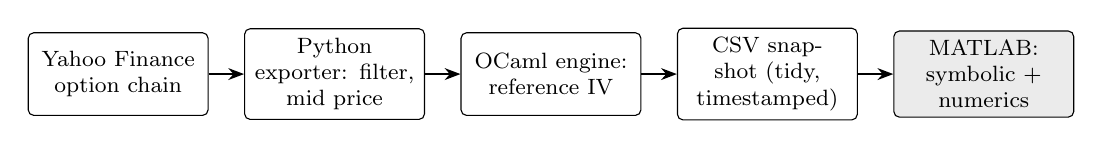
\begin{tikzpicture}[
  node distance=0.45cm,
  box/.style={draw, rounded corners=2pt, minimum height=1.05cm, minimum width=2.15cm,
              text width=2.05cm, align=center, font=\footnotesize},
  arr/.style={-{Stealth[length=2mm]}, thick}]
  \node[box] (yf) {Yahoo Finance option chain};
  \node[box, right=of yf] (py) {Python exporter: filter, mid price};
  \node[box, right=of py] (ml) {OCaml engine: reference IV};
  \node[box, right=of ml] (csv) {CSV snapshot (tidy, timestamped)};
  \node[box, right=of csv, fill=black!8] (mat) {MATLAB: symbolic + numerics};
  \draw[arr] (yf) -- (py);
  \draw[arr] (py) -- (ml);
  \draw[arr] (ml) -- (csv);
  \draw[arr] (csv) -- (mat);
\end{tikzpicture}
\caption{Data flow. The shaded stage is the focus of this project; the earlier stages already exist and are extended by a snapshot exporter. The interactive application sits on top of the MATLAB stage.}
\end{figure}

\section{Methods}

\subsection{Symbolic derivation}
With a continuous dividend yield $q$ (zero reproduces the existing engine exactly), the call and put prices are
\begin{align}
  d_1 &= \frac{\ln(S/K) + (r - q + \tfrac12\sigma^2)T}{\sigma\sqrt{T}}, \qquad d_2 = d_1 - \sigma\sqrt{T},\\
  C &= S e^{-qT}\Phi(d_1) - K e^{-rT}\Phi(d_2), \qquad
  P = K e^{-rT}\Phi(-d_2) - S e^{-qT}\Phi(-d_1),
\end{align}
where $\Phi$ is the standard normal distribution function. The Symbolic Math Toolbox differentiates these expressions to obtain the Greeks, in particular vega $\nu = \partial C/\partial\sigma = S e^{-qT}\varphi(d_1)\sqrt{T}$, and \texttt{matlabFunction} compiles them into vectorised numerical functions. Two identities are checked on the symbolic expressions rather than assumed: the Black--Scholes partial differential equation,
\begin{equation}
  -\frac{\partial C}{\partial T} + (r-q)S\frac{\partial C}{\partial S} + \tfrac12\sigma^2 S^2\frac{\partial^2 C}{\partial S^2} - rC = 0,
\end{equation}
and put--call parity, $C - P = Se^{-qT} - Ke^{-rT}$.

\subsection{Implied volatility solver}
Given a market price $C_{\mathrm{mkt}}$, the solver finds $\sigma$ with $C(\sigma) = C_{\mathrm{mkt}}$ by Newton--Raphson,
\begin{equation}
  \sigma_{n+1} = \sigma_n - \frac{C(\sigma_n) - C_{\mathrm{mkt}}}{\nu(\sigma_n)},
\end{equation}
using the symbolically derived vega. Because the price is strictly increasing in $\sigma$, every iterate also tightens a bracket $[\sigma_{\mathrm{lo}},\sigma_{\mathrm{hi}}]$ (initially $[10^{-4},5]$). If vega is nearly zero or a Newton step leaves the bracket, the step falls back to bisection, which guarantees convergence. A price outside the attainable range, such as one below intrinsic value, returns \texttt{NaN} because it violates no-arbitrage bounds. The method records how often the fallback was needed, which gives a direct comparison of the two root-finding strategies.

A practical limit is \emph{identifiability}: the volatility error is roughly the price tolerance divided by vega, so deep in-the-money and short-dated options, whose prices are almost independent of $\sigma$, cannot yield a reliable $\IV$. This motivates the choice of quotes below.

\subsection{Forward price and quote selection}
Put--call parity implies $F = K + e^{rT}(C - P)$ for any strike with both a call and a put. For each expiry the forward $F$ is taken as the median over the five strikes nearest spot. Only out-of-the-money quotes are used (puts with $K<F$, calls with $K\ge F$), since they carry mostly time value and therefore the most reliable volatility information. Positions are expressed in log-moneyness $k = \ln(K/F)$.

\subsection{Surface construction}
The surface is interpolated in total variance $w(k,T) = \IV^2\,T$, which behaves more regularly across maturities than $\IV$ itself. Both axes are rescaled to $[0,1]$, because $k$ and $T$ differ in scale by an order of magnitude and Delaunay triangulation is scale-sensitive. The interpolant is piecewise linear on the triangulation, with volatility recovered as $\IV = \sqrt{w/T}$. The surface is deliberately \emph{not} extrapolated: outside the convex hull of the data it is undefined, so holes mark regions with no market information. Slices then follow directly: a \emph{smile} fixes $T$ and varies $k$, and a \emph{term structure} fixes $k$ (by default $k=0$, at the forward) and varies $T$.

\subsection{Interactive interface}
An App Designer application will provide a ticker field with a refresh button that runs the Python exporter through MATLAB's Python interface, an expiry selector, the three-dimensional surface with the market quotes overlaid, and linked smile and term-structure panels. Cached snapshots keep the demonstration reproducible when markets are closed or the data feed is unavailable.

\section{Validation}
Correctness is checked at three levels, by automated MATLAB tests where possible.
\begin{itemize}
  \item \textbf{Symbolic checks:} the PDE residual and put--call parity are verified symbolically and numerically at random points.
  \item \textbf{Known-answer tests:} prices generated from known volatilities are inverted to recover them; the surface interpolator is tested against an analytic surface; invalid inputs must be rejected with clear errors.
  \item \textbf{Cross-validation:} MATLAB implied volatilities are compared with the OCaml engine on live data.
\end{itemize}

Preliminary results from the completed components are in Table~\ref{tab:results}. The maximum difference to the OCaml engine, $5\times10^{-7}$, is exactly the rounding error of that engine's output, which is printed to six decimal places; the two solvers therefore agree to the precision the engine reports.

\begin{table}[h]
\centering
\small
\begin{tabular}{@{}p{7.2cm}p{5.6cm}@{}}
\toprule
Check & Result \\
\midrule
Symbolic PDE and put--call parity & proved symbolically; residual $2\times10^{-14}$ numerically \\
Implied-volatility round trip (142 well-posed cases) & worst error $3.1\times10^{-7}$ \\
AAPL snapshot, 12 Oct 2026: 140 OTM contracts, 8 expiries & all converged, no bisection fallback needed \\
Difference from OCaml engine on that snapshot & median $2.6\times10^{-7}$, maximum $5.0\times10^{-7}$ \\
Interpolation error on an analytic surface & below $5\times10^{-4}$ (volatility space), $3.5\times10^{-3}$ (total variance) \\
\bottomrule
\end{tabular}
\caption{Preliminary validation results.}
\label{tab:results}
\end{table}

\section{Scope, limitations and extensions}
\textbf{Limitations.} Listed equity options are American-style, so early-exercise value is ignored by the European model; this matters most for in-the-money options and is one more reason for the out-of-the-money selection. The engine has no dividend term ($q=0$), so the forward is inferred from put--call parity instead. Free market data is delayed and noisy: thinly quoted, short-dated expiries can produce spurious dips in the surface, and a minimum-quotes-per-expiry rule is under consideration. Finally, the interpolated surface is not guaranteed to be free of arbitrage.

\textbf{Extensions (outside this project).} Fitting a parametric smile model to each expiry, such as the SVI parameterisation, together with explicit no-arbitrage checks on strike (butterfly) and maturity (calendar) convexity, would be a natural follow-up and would use this interpolated surface as its baseline.

\section{Status}
\begin{table}[h]
\centering
\small
\begin{tabular}{@{}lc@{}}
\toprule
Component & Status \\
\midrule
Snapshot exporter and CSV format (Python) & Complete \\
Symbolic derivation and implied-volatility solver & Complete \\
Forward estimation and out-of-the-money selection & Complete \\
Surface interpolation, slices and automated tests & Complete \\
Interactive App Designer application & Planned \\
Written report and demonstration & Planned \\
\bottomrule
\end{tabular}
\end{table}

\end{document}
